% !TeX root = 系统动力学建模与仿真笔记.tex
\section{系统广义质量矩阵对时间的一阶导数}

系统广义质量矩阵中 $M_{j,k}^i$ 的时间导数满足
\begin{align}
\dot{M}_{j,k}^i &= \frac{\mathrm{d}}{\mathrm{d}t}\left(\bm{\Phi}_{\mathrm{J}_j}^{\mathrm{T}} \bm{C}_{i,j}^{\mathrm{T}} M_i \bm{C}_{i,k} \bm{\Phi}_{\mathrm{J}_k}\right) \notag \\
&= \left(\dot{\bm{\Phi}}_{\mathrm{J}_j}^{\mathrm{T}} \bm{C}_{i,j}^{\mathrm{T}} + \bm{\Phi}_{\mathrm{J}_j}^{\mathrm{T}} \dot{\bm{C}}_{i,j}^{\mathrm{T}}\right) M_i \bm{C}_{i,k} \bm{\Phi}_{\mathrm{J}_k} + \bm{\Phi}_{\mathrm{J}_j}^{\mathrm{T}} \bm{C}_{i,j}^{\mathrm{T}} M_i \left(\dot{\bm{C}}_{i,k} \bm{\Phi}_{\mathrm{J}_k} + \bm{C}_{i,k} \dot{\bm{\Phi}}_{\mathrm{J}_k}\right),
\tag{11.6}
\end{align}
式中 $\dot{\bm{C}}_{i,k}$ 可通过递推方式获得，即
\begin{equation}
\dot{\bm{C}}_{i,k} = \frac{\mathrm{d}}{\mathrm{d}t}\left(\bm{C}_{i,\mathrm{p}(i)} \bm{C}_{\mathrm{p}(i),k}\right) = \dot{\bm{C}}_{i,\mathrm{p}(i)} \bm{C}_{\mathrm{p}(i),k} + \bm{C}_{i,\mathrm{p}(i)} \dot{\bm{C}}_{\mathrm{p}(i),k},
\tag{11.7}
\end{equation}
\begin{align}
\dot{\bm{C}}_{i,\mathrm{p}(i)} &= \frac{\mathrm{d}}{\mathrm{d}t} \begin{bmatrix}
\bm{A}_{\mathrm{p}(i),i}^{\mathrm{T}} & \bm{A}_{\mathrm{p}(i),i}^{\mathrm{T}} \tilde{\bm{r}}_{\mathrm{O}_{\mathrm{p}(i)}\mathrm{O}_i|\mathrm{p}(i)}^{\mathrm{T}} \\
\bm{O}_3 & \bm{A}_{\mathrm{p}(i),i}^{\mathrm{T}}
\end{bmatrix} \notag \\
&= \begin{bmatrix}
\left(\bm{A}_{\mathrm{p}(i),i} \tilde{\bm{\omega}}_{\mathrm{p}(i),i|i}\right)^{\mathrm{T}} & \bm{A}_{\mathrm{p}(i),i}^{\mathrm{T}} \tilde{\bm{r}}_{\mathrm{O}_{\mathrm{p}(i)}\mathrm{O}_i|\mathrm{p}(i)}^{\mathrm{T}} + \left(\bm{A}_{\mathrm{p}(i),i} \tilde{\bm{\omega}}_{\mathrm{p}(i),i|i}\right)^{\mathrm{T}} \tilde{\bm{r}}_{\mathrm{O}_{\mathrm{p}(i)}\mathrm{O}_i|\mathrm{p}(i)}^{\mathrm{T}} \\
\bm{O}_3 & \left(\bm{A}_{\mathrm{p}(i),i} \tilde{\bm{\omega}}_{\mathrm{p}(i),i|i}\right)^{\mathrm{T}}
\end{bmatrix} \notag \\
&= \begin{bmatrix}
\left(\bm{A}_{\mathrm{p}(i),i} \tilde{\bm{\omega}}_{\mathrm{p}(i),i|i}\right)^{\mathrm{T}} & \bm{A}_{\mathrm{p}(i),i}^{\mathrm{T}} \tilde{\bm{r}}_{\mathrm{R}_i\mathrm{O}_i|\mathrm{p}(i)}^{\mathrm{T}} + \left(\bm{A}_{\mathrm{p}(i),i} \tilde{\bm{\omega}}_{\mathrm{p}(i),i|i}\right)^{\mathrm{T}} \tilde{\bm{r}}_{\mathrm{O}_{\mathrm{p}(i)}\mathrm{O}_i|\mathrm{p}(i)}^{\mathrm{T}} \\
\bm{O}_3 & \left(\bm{A}_{\mathrm{p}(i),i} \tilde{\bm{\omega}}_{\mathrm{p}(i),i|i}\right)^{\mathrm{T}}
\end{bmatrix}.
\tag{11.8}
\end{align}

\section{系统动能对广义坐标的偏导数}

系统动能对广义坐标的偏导数可记为
\begin{equation}
T_q = \left[T_{q_{\mathrm{J}_1}} \quad T_{q_{\mathrm{J}_2}} \quad \cdots \quad T_{q_{\mathrm{J}_{n_s}}}\right],
\tag{11.9}
\end{equation}
其中各分量满足
\begin{equation}
T_{q_{\mathrm{J}_j}} = \frac{\partial}{\partial q_{\mathrm{J}_j}} \left(\frac{1}{2} \sum_{i=1}^n \bm{v}_{0,i|i}^{\mathrm{T}} M_i \bm{v}_{0,i|i}\right) = \sum_{i=1}^n \bm{v}_{0,i|i}^{\mathrm{T}} M_i \frac{\partial \bm{v}_{0,i|i}}{\partial q_{\mathrm{J}_j}}.
\tag{11.10}
\end{equation}

对于 $j \in \bar{\mathrm{p}}[i]$，有
\begin{align}
\frac{\partial \bm{v}_{0,i|i}}{\partial q_{\mathrm{J}_j}} &= \frac{\partial}{\partial q_{\mathrm{J}_j}} \left(\sum_{k \in \bar{\mathrm{p}}[i]} \bm{C}_{i,k} \bm{\Phi}_{\mathrm{J}_k} \dot{q}_{\mathrm{J}_k}\right) = \sum_{k \in \bar{\mathrm{p}}[i]} \frac{\partial}{\partial q_{\mathrm{J}_j}} \left(\bm{C}_{i,k} \bm{\Phi}_{\mathrm{J}_k} \dot{q}_{\mathrm{J}_k}\right) \notag \\
&= \sum_{k \in \bar{\mathrm{p}}[i]} \frac{\partial}{\partial q_{\mathrm{J}_j}} \left(\bm{C}_{i,k} \bm{\Phi}_{\mathrm{J}_k} \dot{q}_{\mathrm{J}_k}\right) + \frac{\partial}{\partial q_{\mathrm{J}_j}} \left(\bm{C}_{i,j} \bm{\Phi}_{\mathrm{J}_j} \dot{q}_{\mathrm{J}_j}\right) \notag \\
&= \sum_{k \in \bar{\mathrm{p}}[j]} \frac{\partial}{\partial q_{\mathrm{J}_j}} \left(\bm{C}_{i,j} \bm{C}_{j,\mathrm{p}(j)} \bm{C}_{\mathrm{p}(j),k} \bm{\Phi}_{\mathrm{J}_k} \dot{q}_{\mathrm{J}_k}\right) + \bm{C}_{i,j} \frac{\partial}{\partial q_{\mathrm{J}_j}} \left(\bm{\Phi}_{\mathrm{J}_j} \dot{q}_{\mathrm{J}_j}\right) \notag \\
&= \sum_{k \in \bar{\mathrm{p}}[j]} \bm{C}_{i,j} \frac{\partial}{\partial q_{\mathrm{J}_j}} \left(\bm{C}_{j,\mathrm{p}(j)} \bm{C}_{\mathrm{p}(j),k} \bm{\Phi}_{\mathrm{J}_k} \dot{q}_{\mathrm{J}_k}\right) + \bm{C}_{i,j} \frac{\partial}{\partial q_{\mathrm{J}_j}} \left(\bm{\Phi}_{\mathrm{J}_j} \dot{q}_{\mathrm{J}_j}\right) \notag \\
&=: \sum_{k \in \bar{\mathrm{p}}[j]} \bm{C}_{i,j} \frac{\partial}{\partial q_{\mathrm{J}_j}} \left(\bm{C}_{j,\mathrm{p}(j)} \bm{v}_{\mathrm{p}(j),k}\right) + \bm{C}_{i,j} \frac{\partial}{\partial q_{\mathrm{J}_j}} \left(\bm{\Phi}_{\mathrm{J}_j} \dot{q}_{\mathrm{J}_j}\right),
\tag{11.11}
\end{align}
式中各系数矩阵与铰元件广义坐标的关系如图11.1所示。

% 图片占位符
\begin{figure}[H]
    \centering
    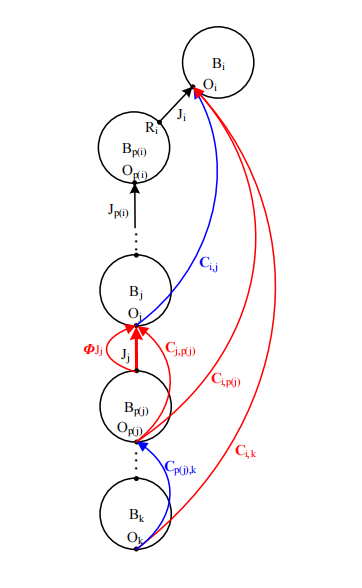
\includegraphics[width=0.8\textwidth]{Figure/PDF/SystemDynamicsModelingAndSimulation_109.png}
    \caption{系统动能对广义坐标的偏导数及连体坐标系速度与铰元件广义坐标的关系}
    \label{fig:chapter11_page95}
\end{figure}

\begin{equation}
\bm{C}_{j,\mathrm{p}(j)} \bm{v}_{\mathrm{p}(j),k} = \begin{bmatrix}
\bm{A}_{\mathrm{p}(j),j}^{\mathrm{T}} & \bm{A}_{\mathrm{p}(j),j}^{\mathrm{T}} \tilde{\bm{r}}_{\mathrm{O}_{\mathrm{p}(j)}\mathrm{O}_j|\mathrm{p}(j)}^{\mathrm{T}} \\
\bm{O}_3 & \bm{A}_{\mathrm{p}(j),j}^{\mathrm{T}}
\end{bmatrix}
\begin{bmatrix}
\bm{v}_{\mathrm{U}} \\
\bm{v}_{\mathrm{D}}
\end{bmatrix}
= \begin{bmatrix}
\bm{A}_{\mathrm{p}(j),j}^{\mathrm{T}} \bm{v}_{\mathrm{U}} + \bm{A}_{\mathrm{p}(j),j}^{\mathrm{T}} \tilde{\bm{v}}_{\mathrm{D}} \bm{r}_{\mathrm{O}_{\mathrm{p}(j)}\mathrm{O}_j|\mathrm{p}(j)} \\
\bm{A}_{\mathrm{p}(j),j}^{\mathrm{T}} \bm{v}_{\mathrm{D}}
\end{bmatrix},
\tag{11.12}
\end{equation}
\begin{align}
\frac{\partial}{\partial q_{\mathrm{J}_j}} \left(\bm{C}_{j,\mathrm{p}(j)} \bm{v}_{\mathrm{p}(j),k}\right) &= \frac{\partial}{\partial q_{\mathrm{J}_j}} \left(\begin{bmatrix}
\bm{A}_{\mathrm{p}(j),j}^{\mathrm{T}} \bm{v}_{\mathrm{U}} + \bm{A}_{\mathrm{p}(j),j}^{\mathrm{T}} \tilde{\bm{v}}_{\mathrm{D}} \bm{r}_{\mathrm{O}_{\mathrm{p}(j)}\mathrm{O}_j|\mathrm{p}(j)} \\
\bm{A}_{\mathrm{p}(j),j}^{\mathrm{T}} \bm{v}_{\mathrm{D}}
\end{bmatrix}\right) \notag \\
&=: \begin{bmatrix}
\frac{\partial}{\partial q_{\mathrm{J}_j}} \left(\bm{A}_{\mathrm{p}(j),j}^{\mathrm{T}} \bm{v}_{\mathrm{U}}\right) + \frac{\partial}{\partial q_{\mathrm{J}_j}} \left(\bm{A}_{\mathrm{p}(j),j}^{\mathrm{T}} \bm{v}_{\mathrm{I}}\right) + \bm{A}_{\mathrm{p}(j),j}^{\mathrm{T}} \tilde{\bm{v}}_{\mathrm{D}} \frac{\partial}{\partial q_{\mathrm{J}_j}} \left(\bm{r}_{\mathrm{O}_{\mathrm{p}(j)}\mathrm{O}_j|\mathrm{p}(j)}\right) \\
\frac{\partial}{\partial q_{\mathrm{J}_j}} \left(\bm{A}_{\mathrm{p}(j),j}^{\mathrm{T}} \bm{v}_{\mathrm{D}}\right)
\end{bmatrix},
\tag{11.13}
\end{align}
式中 $\bm{v}_{\mathrm{I}} = \tilde{\bm{v}}_{\mathrm{D}} \bm{r}_{\mathrm{O}_{\mathrm{p}(j)}\mathrm{O}_j|\mathrm{p}(j)}$，视为与 $q_{\mathrm{J}_j}$ 无关的三维列阵。式中各子雅可比矩阵的表达式见第~\ref{sec:ch11-jiaopian-partial}~节。

\section{铰元件相对运动学量对自身广义坐标的偏导数}\label{sec:ch11-jiaopian-partial}

\parahead{虚拟铰元件}

对于虚拟铰元件 $i$：
\begin{equation}
\frac{\partial}{\partial q_{\mathrm{J}_i}} \left(\bm{r}_{\mathrm{O}_{\mathrm{p}(i)}\mathrm{O}_i|\mathrm{p}(i)}\right) = \begin{bmatrix} \bm{I}_3 & \bm{O}_3 \end{bmatrix},
\tag{11.14}
\end{equation}
\begin{equation}
\frac{\partial}{\partial q_{\mathrm{J}_i}} \left(\bm{A}_{\mathrm{p}(i),i}^{\mathrm{T}} \bm{v}\right) = \begin{bmatrix} \bm{O}_3 & \bm{A}_{\mathrm{p}(i),i}^{\mathrm{T}} \tilde{\bm{v}} \bm{A}_{\mathrm{p}(i),i} \bm{H}_{\mathrm{B321}}(\bm{\theta}_{\mathrm{J}_i}) \end{bmatrix},
\tag{11.15}
\end{equation}
\begin{align}
\frac{\partial}{\partial q_{\mathrm{J}_i}} \left(\bm{\Phi}_{\mathrm{J}_i} \dot{q}_{\mathrm{J}_i}\right) &= \begin{bmatrix}
\frac{\partial}{\partial \bm{l}_{\mathrm{J}_i}} \begin{bmatrix}
\bm{A}_{\mathrm{p}(i),i}^{\mathrm{T}} \dot{\bm{l}}_{\mathrm{J}_i} \\
\bm{H}_{\mathrm{B321}}(\bm{\theta}_{\mathrm{J}_i}) \dot{\bm{\theta}}_{\mathrm{J}_i}
\end{bmatrix} & \frac{\partial}{\partial \bm{\theta}_{\mathrm{J}_i}} \begin{bmatrix}
\bm{A}_{\mathrm{p}(i),i}^{\mathrm{T}} \dot{\bm{l}}_{\mathrm{J}_i} \\
\bm{H}_{\mathrm{B321}}(\bm{\theta}_{\mathrm{J}_i}) \dot{\bm{\theta}}_{\mathrm{J}_i}
\end{bmatrix} \end{bmatrix} \notag \\
&= \begin{bmatrix}
\bm{O}_{6 \times 3} & \begin{bmatrix}
\bm{A}_{\mathrm{p}(i),i}^{\mathrm{T}} \tilde{\bm{l}}_{\mathrm{J}_i} \bm{A}_{\mathrm{p}(i),i} \bm{H}_{\mathrm{B321}}(\bm{\theta}_{\mathrm{J}_i}) \\
\frac{\partial}{\partial \bm{\theta}_{\mathrm{J}_i}} \left(\bm{H}_{\mathrm{B321}} \dot{\bm{\theta}}_{\mathrm{J}_j}\right)
\end{bmatrix} \end{bmatrix},
\tag{11.16}
\end{align}
\begin{equation}
\frac{\partial}{\partial \bm{\theta}} \left(\bm{H}_{\mathrm{B321}} \dot{\bm{\theta}}\right) = \begin{bmatrix}
0 & -c_2 \dot{\theta}_1 & 0 \\
0 & -s_2 s_3 \dot{\theta}_1 & c_2 c_3 \dot{\theta}_1 - s_3 \dot{\theta}_2 \\
0 & -s_2 c_3 \dot{\theta}_1 & -c_2 s_3 \dot{\theta}_1 - c_3 \dot{\theta}_2
\end{bmatrix}.
\tag{11.17}
\end{equation}
式中 $c_2 = \cos(\theta_2)$, $s_2 = \sin(\theta_2)$, $c_3 = \cos(\theta_3)$, $s_3 = \sin(\theta_3)$。

\parahead{转动铰元件}

对于转动铰元件 $i$：
\begin{equation}
\frac{\partial}{\partial q_{\mathrm{J}_i}} \left(\bm{r}_{\mathrm{O}_{\mathrm{p}(i)}\mathrm{O}_i|\mathrm{p}(i)}\right) = \bm{0}_3,
\tag{11.18}
\end{equation}
\begin{equation}
\frac{\partial}{\partial q_{\mathrm{J}_i}} \left(\bm{A}_{\mathrm{p}(i),i}^{\mathrm{T}} \bm{v}\right) = \bm{A}_{\mathrm{p}(i),i}^{\mathrm{T}} \tilde{\bm{v}} \bm{A}_{\mathrm{p}(i),i} \bm{n}_{\mathrm{J}_i} = \bm{A}_{\mathrm{p}(i),i}^{\mathrm{T}} \tilde{\bm{v}} \bm{n}_{\mathrm{J}_i},
\tag{11.19}
\end{equation}
\begin{equation}
\frac{\partial}{\partial q_{\mathrm{J}_i}} \left(\bm{\Phi}_{\mathrm{J}_i} \dot{q}_{\mathrm{J}_i}\right) = \bm{0}_6.
\tag{11.20}
\end{equation}

\section{加速度约束方程}

闭环 $\mathrm{L}_j$ 切断铰加速度级约束方程可表示为
\begin{align}
\bm{0} = \ddot{c}_{\mathrm{L}_j} &= \frac{\mathrm{d}}{\mathrm{d}t} \dot{c}_{\mathrm{L}_j} \notag \\
&= \frac{\mathrm{d}}{\mathrm{d}t} \left(c_{\mathrm{L}_j,q} \dot{q} + c_{\mathrm{L}_j,t}\right) \notag \\
&=: c_{\mathrm{L}_j,q} \ddot{q} + \dot{c}_{\mathrm{L}_j,q} \dot{q} + \dot{c}_{\mathrm{L}_j,t}.
\tag{11.21}
\end{align}

对于转动铰
\begin{equation}
c_{\mathrm{L}_j,t} = \bm{0},
\tag{11.22}
\end{equation}
\begin{equation}
\dot{c}_{\mathrm{L}_j,t} = \bm{0}.
\tag{11.23}
\end{equation}

当 $k \in \bar{\mathrm{p}}[\underline{\mathrm{m}}(j)]$ 且 $k > \underline{\mathrm{r}}(j)$ 时，
\begin{align}
\frac{\mathrm{d}}{\mathrm{d}t} c_{\mathrm{L}_j,q_{\mathrm{J}_k}} &= \frac{\mathrm{d}}{\mathrm{d}t} \left(\bm{\Psi}_{\underline{\mathrm{m}}(j)} \bm{C}_{\underline{\mathrm{m}}(j),k} \bm{\Phi}_{\mathrm{J}_k}\right) \notag \\
&= \dot{\bm{\Psi}}_{\underline{\mathrm{m}}(j)} \bm{C}_{\underline{\mathrm{m}}(j),k} \bm{\Phi}_{\mathrm{J}_k} + \bm{\Psi}_{\underline{\mathrm{m}}(j)} \dot{\bm{C}}_{\underline{\mathrm{m}}(j),k} \bm{\Phi}_{\mathrm{J}_k} + \bm{\Psi}_{\underline{\mathrm{m}}(j)} \bm{C}_{\underline{\mathrm{m}}(j),k} \dot{\bm{\Phi}}_{\mathrm{J}_k};
\tag{11.24}
\end{align}
当 $k \in \bar{\mathrm{p}}[\underline{\mathrm{b}}(j)]$ 且 $k > \underline{\mathrm{r}}(j)$ 时，
\begin{align}
\frac{\mathrm{d}}{\mathrm{d}t} c_{\mathrm{L}_j,q_{\mathrm{J}_k}} &= \frac{\mathrm{d}}{\mathrm{d}t} \left(-\bm{\Psi}_{\underline{\mathrm{b}}(j)} \bm{C}_{\underline{\mathrm{b}}(j),k} \bm{\Phi}_{\mathrm{J}_k}\right) \notag \\
&= -\dot{\bm{\Psi}}_{\underline{\mathrm{b}}(j)} \bm{C}_{\underline{\mathrm{b}}(j),k} \bm{\Phi}_{\mathrm{J}_k} - \bm{\Psi}_{\underline{\mathrm{b}}(j)} \dot{\bm{C}}_{\underline{\mathrm{b}}(j),k} \bm{\Phi}_{\mathrm{J}_k} - \bm{\Psi}_{\underline{\mathrm{b}}(j)} \bm{C}_{\underline{\mathrm{b}}(j),k} \dot{\bm{\Phi}}_{\mathrm{J}_k}.
\tag{11.25}
\end{align}

\section{与非切断铰元件绑定的弹性阻尼力与控制力}\label{sec:ch11-noncut-force}

与非切断铰元件，如铰元件 $\mathrm{J}_k$，绑定的线弹性阻尼力与控制力对应的广义力可表示为
\begin{equation}
\bm{f}_{\mathrm{J}_k} = -\bm{K}_{\mathrm{P},\mathrm{J}_k}(\bm{q}_{\mathrm{J}_k} - \bar{\bm{q}}_{\mathrm{J}_k}) - \bm{K}_{\mathrm{D},\mathrm{J}_k} \dot{\bm{q}}_{\mathrm{J}_k} + \bm{f}_{\mathrm{C},\mathrm{J}_k},
\tag{11.26}
\end{equation}
式中 $\bm{K}_{\mathrm{P},\mathrm{J}_k}$ 与 $\bm{K}_{\mathrm{D},\mathrm{J}_k}$ 分别为由铰元件 $\mathrm{J}_k$ 刚度系数与阻尼系数形成的对角矩阵，$\bar{\bm{q}}_{\mathrm{J}_k}$ 为弹性/扭簧发挥作用的起始位置，$\bm{f}_{\mathrm{C},\mathrm{J}_k}$ 为铰元件控制力/力矩。

\section{其它系统广义力}

除了第~\ref{sec:ch11-noncut-force}~节讨论的与非切断铰元件绑定的弹性阻尼力与控制力，系统受到的其它弹性阻尼力、摩擦力、控制力与重力作如下统一处理：
\begin{enumerate}
\item 将这些力等效到相应的体元件，若为刚体则等效到体元件连体坐标系，
\item 将等效到体元件上的力转为系统广义力。
\end{enumerate}

将等效在体元件 $i$ 连体坐标系上的力在其连体坐标系中的投影记为
\begin{equation}
\bm{f}_{\mathrm{B}_i} \triangleq \begin{bmatrix}
\bm{\sigma}_{\mathrm{B}_i|i} \\
\bm{\tau}_{\mathrm{O}_i|i}
\end{bmatrix},
\tag{11.27}
\end{equation}
考虑到式~\eqref{eq:10.37}，即
\begin{equation}
\bm{v}_{0,i|i} = \sum_{k \in \bar{\mathrm{p}}[i]} \bm{C}_{i,k} \bm{\Phi}_{\mathrm{J}_k} \dot{q}_{\mathrm{J}_k},
\tag{11.28}
\end{equation}
可知：当 $k \in \bar{\mathrm{p}}[i]$ 时，$\bm{f}_{\mathrm{B}_i}$ 对应的广义力可表示
\begin{equation}
\bm{f}_{\mathrm{J}_k} = \bm{\Phi}_{\mathrm{J}_k}^{\mathrm{T}} \bm{C}_{i,k}^{\mathrm{T}} \bm{f}_{\mathrm{B}_i}
\tag{11.29}
\end{equation}

\section{动力学微分代数方程的约化}

\parahead{独立广义坐标与非独立广义坐标的划分}

下面考虑如何将动力学微分代数方程，即
\begin{equation}
\begin{bmatrix}
\bm{M} & \bm{c}_q^{\mathrm{T}} \\
\bm{c}_q & \bm{O}
\end{bmatrix}
\begin{bmatrix}
\ddot{\bm{q}} \\
\bm{\lambda}
\end{bmatrix}
=
\begin{bmatrix}
\bm{h}(\bm{q}, \dot{\bm{q}}, t) \\
\bm{\varepsilon}(\bm{q}, \dot{\bm{q}}, t)
\end{bmatrix},
\end{equation}
约化为一组二阶常微分方程。

针对四足机器人动力学系统，由于系统的位形可由$\{q_{\mathrm{J}_1}, q_{\mathrm{J}_2}, \cdots, q_{\mathrm{J}_{13}}\}$完全确定，并且$\{q_{\mathrm{J}_1}, q_{\mathrm{J}_2}, \cdots, q_{\mathrm{J}_{13}}\}$相互独立，因此可将$\{q_{\mathrm{J}_1}, q_{\mathrm{J}_2}, \cdots, q_{\mathrm{J}_{13}}\}$称为系统独立广义坐标。系统约束方程$\bm{0} = c(\bm{q}) \in \mathbb{R}^{20}$的作用可以理解为用来确定系统非独立广义坐标$\{q_{\mathrm{J}_{14}}, q_{\mathrm{J}_{15}}, \cdots, q_{\mathrm{J}_{21}}\}$与系统独立广义坐标$\{q_{\mathrm{J}_1}, q_{\mathrm{J}_2}, \cdots, q_{\mathrm{J}_{13}}\}$的关系；系统广义速度和广义加速度亦是如此。若记
\begin{equation}
\begin{bmatrix}
q_{\mathrm{J}_1} \\
q_{\mathrm{J}_2} \\
\vdots \\
q_{\mathrm{J}_{13}}
\end{bmatrix}
=: \bm{q}_{\mathrm{I}} \in \mathbb{R}^{18},
\qquad
\begin{bmatrix}
q_{\mathrm{J}_{14}} \\
q_{\mathrm{J}_{15}} \\
\vdots \\
q_{\mathrm{J}_{21}}
\end{bmatrix}
=: \bm{q}_{\mathrm{D}} \in \mathbb{R}^{8},
\tag{11.30}
\end{equation}
则有
\begin{equation}
\bm{q} = \begin{bmatrix} \bm{q}_{\mathrm{I}} \\ \bm{q}_{\mathrm{D}} \end{bmatrix},
\quad
\dot{\bm{q}} = \begin{bmatrix} \dot{\bm{q}}_{\mathrm{I}} \\ \dot{\bm{q}}_{\mathrm{D}} \end{bmatrix},
\quad
\ddot{\bm{q}} = \begin{bmatrix} \ddot{\bm{q}}_{\mathrm{I}} \\ \ddot{\bm{q}}_{\mathrm{D}} \end{bmatrix},
\tag{11.31}
\end{equation}
当然，这并不是一般的情形；对于更一般的情形，此处暂不讨论。

\parahead{加速度约束方程的整理}

应用系统广义坐标的划分，可将系统加速度级约束方程重新整理为
\begin{align}
\bm{\varepsilon}(\bm{q}, \dot{\bm{q}}, t) &= \bm{c}_q \ddot{\bm{q}} \notag \\
&=: \begin{bmatrix} \bm{c}_{q_{\mathrm{I}}} & \bm{c}_{q_{\mathrm{D}}} \end{bmatrix}
\begin{bmatrix} \ddot{\bm{q}}_{\mathrm{I}} \\ \ddot{\bm{q}}_{\mathrm{D}} \end{bmatrix} \notag \\
&= \bm{c}_{q_{\mathrm{I}}} \ddot{\bm{q}}_{\mathrm{I}} + \bm{c}_{q_{\mathrm{D}}} \ddot{\bm{q}}_{\mathrm{D}}.
\tag{11.32}
\end{align}
考虑到四足机器人系统中存在冗余约束，$\bm{c}_{q_{\mathrm{D}}} \in \mathbb{R}^{20 \times 8}$不是方阵，上式左右两端同时左乘$\bm{c}_{q_{\mathrm{D}}}^{\mathrm{T}}$，整理可得
\begin{equation}
\bm{c}_{q_{\mathrm{D}}}^{\mathrm{T}} \bm{c}_{q_{\mathrm{D}}} \ddot{\bm{q}}_{\mathrm{D}} = -\bm{c}_{q_{\mathrm{D}}}^{\mathrm{T}} \bm{c}_{q_{\mathrm{I}}} \ddot{\bm{q}}_{\mathrm{I}} + \bm{c}_{q_{\mathrm{D}}}^{\mathrm{T}} \bm{\varepsilon}.
\tag{11.33}
\end{equation}
由上式可得
\begin{equation}
\ddot{\bm{q}}_{\mathrm{D}} = -\left(\bm{c}_{q_{\mathrm{D}}}^{\mathrm{T}} \bm{c}_{q_{\mathrm{D}}}\right)^{-1} \bm{c}_{q_{\mathrm{D}}}^{\mathrm{T}} \bm{c}_{q_{\mathrm{I}}} \ddot{\bm{q}}_{\mathrm{I}} + \left(\bm{c}_{q_{\mathrm{D}}}^{\mathrm{T}} \bm{c}_{q_{\mathrm{D}}}\right)^{-1} \bm{c}_{q_{\mathrm{D}}}^{\mathrm{T}} \bm{\varepsilon}.
\tag{11.34}
\end{equation}
则有
\begin{align}
\ddot{\bm{q}} = \begin{bmatrix} \ddot{\bm{q}}_{\mathrm{I}} \\ \ddot{\bm{q}}_{\mathrm{D}} \end{bmatrix}
&= \begin{bmatrix} \bm{I}_{18} \\ -\left(\bm{c}_{q_{\mathrm{D}}}^{\mathrm{T}} \bm{c}_{q_{\mathrm{D}}}\right)^{-1} \bm{c}_{q_{\mathrm{D}}}^{\mathrm{T}} \bm{c}_{q_{\mathrm{I}}} \end{bmatrix} \ddot{\bm{q}}_{\mathrm{I}}
+ \begin{bmatrix} \bm{0}_{18} \\ \left(\bm{c}_{q_{\mathrm{D}}}^{\mathrm{T}} \bm{c}_{q_{\mathrm{D}}}\right)^{-1} \bm{c}_{q_{\mathrm{D}}}^{\mathrm{T}} \bm{\varepsilon} \end{bmatrix} \notag \\
&=: \bm{\Phi} \ddot{\bm{q}}_{\mathrm{I}} + \bm{\xi}.
\tag{11.35}
\end{align}

\parahead{动力学方程的约化}

将式(11.35)代入动力学拉格朗日方程可得
\begin{align}
\bm{h}(\bm{q}, \dot{\bm{q}}, t) &= \bm{M} \ddot{\bm{q}} + \bm{c}_q^{\mathrm{T}} \bm{\lambda} \notag \\
&= \bm{M}(\bm{\Phi} \ddot{\bm{q}}_{\mathrm{I}} + \bm{\xi}) + \bm{c}_q^{\mathrm{T}} \bm{\lambda} \notag \\
&= \bm{M} \bm{\Phi} \ddot{\bm{q}}_{\mathrm{I}} + \bm{M} \bm{\xi} + \bm{c}_q^{\mathrm{T}} \bm{\lambda}.
\tag{11.36}
\end{align}
上式左乘$\bm{\Phi}^{\mathrm{T}}$可得
\begin{equation}
\bm{\Phi}^{\mathrm{T}} \bm{h} = \bm{\Phi}^{\mathrm{T}} \bm{M} \bm{\Phi} \ddot{\bm{q}}_{\mathrm{I}} + \bm{\Phi}^{\mathrm{T}} \bm{M} \bm{\xi} + \bm{\Phi}^{\mathrm{T}} \bm{c}_q^{\mathrm{T}} \bm{\lambda}.
\tag{11.37}
\end{equation}
考虑到
\begin{equation}
\bm{\Phi}^{\mathrm{T}} \bm{c}_q^{\mathrm{T}} \bm{\lambda} = \bm{0},
\tag{11.38}
\end{equation}
式(11.37)可化简为如下二阶常微分方程组
\begin{equation}
\bm{\Phi}^{\mathrm{T}} \bm{M} \bm{\Phi} \ddot{\bm{q}}_{\mathrm{I}} = \bm{\Phi}^{\mathrm{T}} (\bm{h} - \bm{M} \bm{\xi}).
\tag{11.39}
\end{equation}

% 以下两张图为原书第 99—100 页扫描截图，其内容已由上文公式完整转写覆盖，暂作留档：
% \begin{figure}[H]
%     \centering
%     \includegraphics[width=0.8\textwidth]{Figure/PDF/SystemDynamicsModelingAndSimulation_113.png}
%     \caption{动力学微分代数方程的约化——广义坐标划分与加速度约束方程整理（原书第99页）}
%     \label{fig:chapter11_page99}
% \end{figure}
%
% \begin{figure}[H]
%     \centering
%     \includegraphics[width=0.8\textwidth]{Figure/PDF/SystemDynamicsModelingAndSimulation_114.png}
%     \caption{动力学微分代数方程的约化——二阶常微分方程组的推导（原书第100页）}
%     \label{fig:chapter11_page100}
% \end{figure}
